%
%  THESISBOEK
%
%  Dit bestand zorgt voor algemene (layout)definities, en groepeert de
%  afzonderlijke LaTeX-files tot een geheel.
%
%  @author Erwin Six, David De Reu, Brecht Vermeulen
%

\documentclass[11pt,a4paper,oneside,notitlepage]{book}
\usepackage[english,dutch]{babel}

% marges aanpassen
% (opmerking: moet *voor* inclusie van fancyhdr package komen)
\setlength{\hoffset}{-1in}
\setlength{\voffset}{-1in}
\setlength{\topmargin}{2cm}
\setlength{\headheight}{0.5cm}
\setlength{\headsep}{1cm}
\setlength{\oddsidemargin}{3.5cm}
\setlength{\evensidemargin}{3.5cm}
\setlength{\textwidth}{16cm}
\setlength{\textheight}{23.3cm}
\setlength{\footskip}{1.5cm}

\usepackage{fancyhdr}
\usepackage{graphicx}
\usepackage{subfig}
\graphicspath{{figuren/}} % De plaats waar latex zijn figuren gaat halen.
% \usepackage[colorlinks]{hyperref}
\usepackage{url}
\usepackage{amsmath}

\usepackage{hyperref}
\usepackage[toc]{glossaries}
\newacronym{gcd}{GCD}{Greatest Common Divisor}

\makeglossaries

\usepackage{algpseudocode}
\usepackage{algorithm}

\usepackage{listings} 
\usepackage{color}
\definecolor{lightgray}{rgb}{.9,.9,.9}
\definecolor{darkgray}{rgb}{.4,.4,.4}
\definecolor{purple}{rgb}{0.65, 0.12, 0.82}
\lstdefinelanguage{JavaScript}{
  keywords={break, case, catch, continue, debugger, default, delete, do, else, finally, for, function, if, in, instanceof, new, return, switch, this, throw, try, typeof, var, void, while, with},
  morecomment=[l]{//},
  morecomment=[s]{/*}{*/},
  morestring=[b]',
  morestring=[b]",
  ndkeywords={class, export, boolean, throw, implements, import, this},
  keywordstyle=\color{blue}\bfseries,
  ndkeywordstyle=\color{darkgray}\bfseries,
  identifierstyle=\color{black},
  commentstyle=\color{purple}\ttfamily,
  %stringstyle=\color{red}\ttfamily,
  sensitive=true
}

\lstset{
   language=JavaScript,
   extendedchars=true,
   basicstyle=\footnotesize\ttfamily,
   showstringspaces=false,
   showspaces=false,
   %numbers=left,
   numberstyle=\footnotesize,
   numbersep=9pt,
   tabsize=2,
   breaklines=true,
   showtabs=false,
   captionpos=b,
   belowcaptionskip=1\baselineskip,
   frame=L,
   xleftmargin=\parindent,
   language=[x86masm]Assembler,
   basicstyle=\footnotesize\ttfamily,
   commentstyle=\itshape\color{black}
}

\pagestyle{fancy}

\renewcommand{\chaptermark}[1]{\markright{\MakeUppercase{#1}}}
\renewcommand{\sectionmark}[1]{\markright{\thesection~#1}}

\newcommand{\headerfmt}[1]{\textsl{\textsf{#1}}}
\newcommand{\headerfmtpage}[1]{\textsf{#1}}

\fancyhf{}
\fancyhead[LE,RO]{\headerfmtpage{\thepage}}
\fancyhead[LO]{\headerfmt{\rightmark}}
\fancyhead[RE]{\headerfmt{\leftmark}}
\renewcommand{\headrulewidth}{0.5pt}
\renewcommand{\footrulewidth}{0pt}

\fancypagestyle{plain}{ % eerste bladzijde van een hoofdstuk
  \fancyhf{}
  \fancyhead[LE,RO]{\headerfmtpage{\thepage}}
  \fancyhead[LO]{\headerfmt{\rightmark}}
  \fancyhead[RE]{\headerfmt{\leftmark}}
  \renewcommand{\headrulewidth}{0.5pt}
  \renewcommand{\footrulewidth}{0pt}
}

% anderhalve interlinie (opm: titelblad gaat uit van 1.5)
\renewcommand{\baselinestretch}{1.5}

% indien LaTeX niet goed splitst, neem je woord hierin op, of evt om splitsen 
% te voorkomen
\hyphenation{ditmagnooitgesplitstworden dit-woord-splitst-hier}

\begin{document}

% titelblad (voor kaft)
\include{titel}

% lege pagina (!!)

% titelblad (!!)

% geen paginanummering tot we aan de inhoudsopgave komen
\pagestyle{empty}

% voorwoord met dankwoord en toelating tot bruikleen (ondertekend)
%  Voorwoord (dankwoord) en toelating tot bruikleen

\newpage

\noindent \textbf{\huge Voorwoord}

\vspace{1.5cm}

\noindent
Hier komt wat tekst.

\addvspace{4cm}

\noindent Brecht Van de Vyvere, januari 2016\newpage

\noindent \textbf{\huge Toelating tot bruikleen}

\vspace{1.5cm}

\noindent
``De auteur geeft de toelating deze scriptie voor consultatie beschikbaar
te stellen en delen van de scriptie te kopi\"eren voor persoonlijk
gebruik.\\
Elk ander gebruik valt onder de beperkingen van het auteursrecht,
in het bijzonder met betrekking tot de verplichting de bron uitdrukkelijk
te vermelden bij het aanhalen van resultaten uit deze scriptie.''

\addvspace{4cm}

\noindent Brecht Van de Vyvere, januari 2016


% overzicht
%  Overzichtsbladzijde met samenvatting

\newpage

{
\setlength{\baselineskip}{14pt}
\setlength{\parindent}{0pt}
\setlength{\parskip}{8pt}

\begin{center}

\noindent \textbf{\huge
Optimalisatie van client-side\\[8pt]
intermodale routeplanning
}

door 

Brecht Van de Vyvere

Scriptie ingediend tot het behalen van de academische graad van\\
Master of Science in de industri\"ele wetenschappen: informatica

Promotor: Prof.~Erik~Mannens, Prof.~Rik~Van de Walle\\
Scriptiebegeleider: Dr.~Ir.~Ruben~Verborgh, Ing.~Pieter~Colpaert

Vakgroep Elektronica en Informatiesystemen, Vakgroep Industri\"ele Technologie en Constructie\\
Voorzitter: Prof.~Dr.~Ir.~Rik~Van de Walle\\
Faculteit Ingenieurswetenschappen en Architectuur\\
Academiejaar 2015--2016


\end{center}

\section*{Samenvatting}

% TODO: samenvatting

Routeplanning is niet meer weg te denken uit ons dagelijks leven. Is het nu voor de trein naar het werk te nemen of het vliegtuig naar je vakantiebestemming, de mogelijkheden zijn onbeperkt. Sinds enkele jaren wordt transportdata gepubliceerd volgens General Transit Feed Specification (GTFS). Dankzij deze uniforme structuur kunnen er algoritmes bedacht worden om data te combineren en intermodaliteit toe te laten. Bestaande oplossingen maken gebruik van een webservice die zoveel mogelijk vragen van de gebruiker probeert te beantwoorden, maar deze manier is moeilijk uitbreidbaar. \textit{Linked Connections} biedt hier een antwoord op door routeplanning mogelijk te maken op basis van gepubliceerde data. Doordat de server enkel verantwoordelijk is voor het publiceren van connecties is deze makkelijk uitbreidbaar via hypermedia. De cli\"ent berekent zelf welke data nodig is om een om een bepaalde route te kunnen plannen rekening houdend met de eisen van de gebruiker. De huidige implementatie van Linked Connections laat enkel filtering in de tijd toe waardoor de snelheid van het algoritme aan banden ligt. Deze masterproef introduceert een optimalisatie voor routeplanning met Linked Connections.

\section*{Trefwoorden}

% TODO: trefwoorden

Linked Connections, routeplanning, optimalisatie, GTFS

}

\newpage % strikt noodzakelijk om een header op deze blz. te vermijden


\pagestyle{fancy}
\frontmatter

% inhoudstafel
\tableofcontents

% opmaak voor het eigenlijke boek; onderstaande lijnen
% weglaten als de eerste regel van een nieuwe alinea moet
% inspringen in plaats van extra tussenruimte
%\setlength{\parindent}{0pt}
%\setlength{\parskip}{0.5\baselineskip plus 0.5ex minus 0.2ex}
%\setlength{\parskip}{1ex plus 0.5ex minus 0.2ex}

% hoofdstukken
\mainmatter

% hier worden de hoofdstukken ingevoegd (\includes)

\chapter{Inleiding}

Routeplanning is momenteel een van de moeilijkste onderzoeksonderwerpen. Dit komt hoofdzakelijk door twee problemen:

\begin{itemize}
\item Een eerste probleem is dat de data moet bestaan. Zo heeft de Belgische spoorwegennetwerk pas in 2015 hun tijdstabellen opgesteld in een uniform formaat.  Om 100\% correcte routeplanning te doen is realtime informatie noodzakelijk. Er zijn maar zeer weinig ov-bedrijven die dit hebben in het juiste formaat en nog minder die dit vrijgegeven.
\item Een twee probleem hierbij is dat deze data geen Open Data is. Sinds augustus 2015 is de Belgische overheid "open-by-default". Dit houdt in dat alle gegevens van de overheid publiek moeten zijn, tenzij explicitiet verklaard wordt waarom deze niet open kan, bijvoorbeeld wegens privacy-schending. Sommige ov-bedrijven zoals De Lijn en de NMBS, geven hun tijdstabellen pas vrij onder 1 op 1 contract waardoor het voor ontwikkelaars moeilijk is om met deze data aan de slag te gaan.\end{itemize}

Deze twee problemen zorgen ervoor dat het zeer moeilijk is om een oplossing te vinden die duurzaam met deze verschillende datasets kan omgaan.

Er komt meer bij routeplanning kijken dan van punt A naar B te geraken via de snelste of kortste weg. We leven in een wereld vol verandering. Nieuwe technologi\"en zoals the Internet Of Things (IOT) zorgen voor nieuwe opportuniteiten. Meer en meer zal data over jou en jouw omgeving een centrale rol spelen. Ook bij routeplanning is personalisatie belangrijk. Dit kan gaan van interessante gebouwen in de buurt tot toegankelijkheid van perrons voor minder valide mensen.

Open Data is sinds kort in een sterke opmars. Zo is er geschat \footnote{http://www.decroo.belgium.be/nl/groen-licht-voor-federale-open-data-strategie-overheidsdata-voortaan-vrij-beschikbaar} dat Belgi\"e een nettowinst van 900 miljoen euro ontloopt door bepaalde datasets niet open te stellen. Er komt een bewustzijn dat het duurzaam oplossen van bepaalde problemen met data moet gebeuren. 

\section{Probleemstelling}
\label{probleemstelling}

Tot voor kort waren er twee mogelijkheden om een routeplanning applicatie te bouwen:
\begin{itemize}
\item ofwel beschikt de cli\"ent over alle data lokaal. Zo kunnen alle behoeften van de cli\"ent voldaan worden. Dit is kostelijk voor de cli\"ent, want alles moet zelf berekend worden. Meestal bevat deze niet over de nodige geheugencapaciteit om routes te berekenen over grote datasets.
\item ofwel wordt er een server opgezet die een bepaalde functionaliteiten aanbiedt, dit onder de vorm van een  Application Programming Interface (API). Zoals je kan zien in \ref{klassieke-webservice-interface} kunnen er meerdere parameters meegegeven worden: waar is het startpunt, wanneer wil je vertrekken, waar wil je aankomen...
\begin{lstlisting}[label=klassieke-webservice-interface,caption=Klassieke webservice interface]
http://my-api.org?start={...}&bestemming={...}&vertrektijd={?}&transportmodes={...}&extraFeature={...}&...
\end{lstlisting}
Er zijn tiental mogelijke modes zoals de bus, boot of trein. Een andere uitdaging van routeplanning is het overstappen tussen twee perrons. Overstappen is voor een bejaarde niet hetzelfde als voor een marathon-loper. Kortom, routeplanning moet met meerdere factoren rekening kunnen houden. Om dit allemaal te berekenen wordt ervoor geopteerd om de server deze berekeningen te laten doen.
Enkele voordelen hiervan:
\begin{itemize}
\item Cli\"ents met weinig rekenkracht kunnen snel routeplanningsadvies bekomen.
\item Er is weinig bandbreedte nodig: 1 HTTP request is voldoende.
\end{itemize}
Er zijn ook enkele nadelen hieraan verbonden:
\begin{itemize}
\item Personalisatie is zeer moeilijk.
\item Een service uitbreiden is moeizaam door de vele factoren die mee rekening gehouden worden.\end{itemize}
\end{itemize}

In figuur \ref{probleemrouteplanning} zie je deze mogelijkheden weergegeven op een Linked Data Fragments-as (LDF). Dit is een conceptueel framework om de balans tussen cli\"ent en server weer te geven. Later (\ref{ldf}) zal dit beter uitgelegd worden.
 \begin{figure}[h!]
\centering
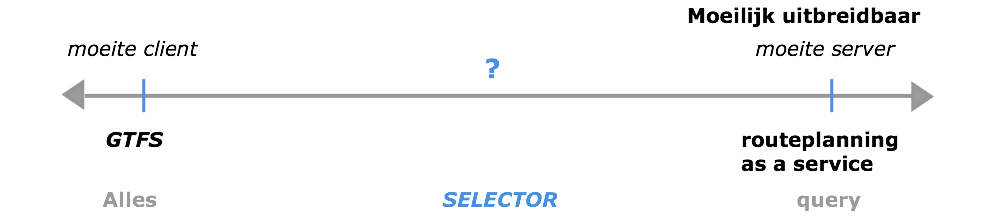
\includegraphics[width=0.8\textwidth]{LDF-as2.png}
\caption{Linked Data Fragments as: huidige oplossingen om routes te plannen. Cli\"ent beschikken ofwel over alle data in een dump, ofwel over een service die het routeplannen voor zich neemt.}
\label{probleemrouteplanning}
\end{figure}

Linked Connections is een manier om transportdata te publiceren zodanig dat het mogelijk is om een route te berekenen hieruit. De basiseenheid is een connectie (zie \ref{connectievb}). Een connectie is de verbinding tussen een vertrek- en eindstop zonder onderbreking, met respectievelijk een vertrek- en aankomsttijd. Een route bestaat uit een combinatie van deze connecties. Connecties zijn gelinkt als ze links bevatten naar andere informatie, zoals connecties die hierop volgen of interessante koffiebars in de buurt.

\begin{figure}[h!]
\centering
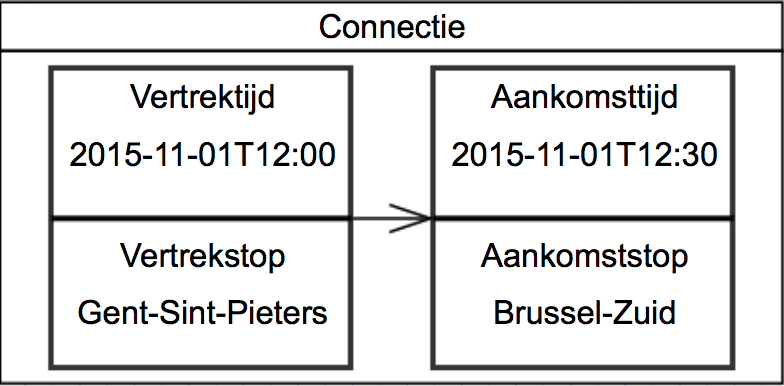
\includegraphics[scale=0.5]{connectie.png}
\caption{Voorbeeld van een connectie. Deze bestaat uit een vertrek- en aankomstplaats, resp. met vertrek- en aankomsttijd}
\label{connectievb}
\end{figure}

Met Linked Connections is het mogelijk om client-side een route te berekenen terwijl server-side connecties ter beschikking stelt. Dit introduceert nieuwe trade-offs die onderzocht kunnen worden. Deze worden weergegeven op de LDF-as \ref{LDF-as3.png}

 \begin{figure}[h!]
\centering
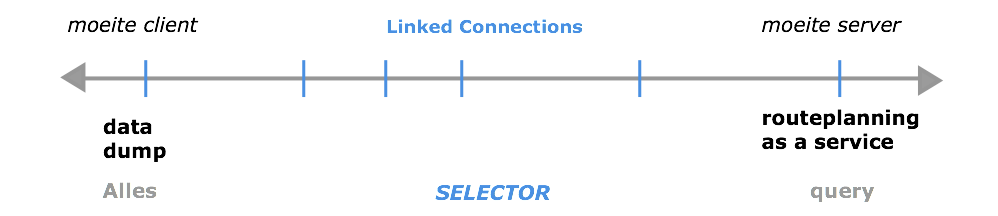
\includegraphics[width=0.8\textwidth]{LDF-as3.png}
\caption{Linked Connections opent nieuwe trade-offs tussen cli\"ent en server aan.}
\label{probleemrouteplanning}
\end{figure}

%\vspace{3mm} %5mm vertical space

De bestaande Linked Connections implementatie werkt momenteel enkel voor een server die connecties ter beschikking stelt. Een probleem hierbij is dat connecties enkel opvraagbaar zijn binnen een tijdsinterval. De cli\"ent wordt overstelpt met connecties die niet nuttig zijn voor het berekenen van de route.

Het doel van deze masterproef is te onderzoeken hoe meerdere datastromen van connecties samengebundeld kunnen worden. Vervolgens wordt onderzocht wat de performantie met de huidige implementatie is en hoe deze verbeterd kan worden.

\section{Onderzoeksvraag}

Deze masterproef zal hoofdzakelijk een antwoord bieden op volgende vraag:
\begin{itemize}
\item \emph{Hoe kunnen we client-side routeplannen met gelinkte connecties sneller maken?}
\end{itemize}

Client-side routeplannen kan sowieso sneller gemaakt worden zoals bij huidige routeplanners het geval is. We willen alle mogelijkheden van het web gebruiken om het publiceren van die gelinkte connecties op de server zo kosteloos mogelijk te maken met daarbij enkele filtermogelijkheden om het routeplannen op de client snel te maken. Verschillende \textit{trade-offs} zullen onderzocht moeten worden.

Enkele subvragen die we hierbij kunnen stellen, zijn:
\begin{enumerate}
\item Welke extra filter(s) moeten toegevoegd worden?
\item Welke metadata kan een meerwaarde bieden voor de cli\"ent?
\item Kunnen we garanderen dat de snelste route gevonden wordt bij extra filtering?
\item Wat is het effect van caching op de berekeningstijd?
\end{enumerate}

\section{Hypotheses}
\label{hypotheses}
Volgende hypotheses zijn waargenomen:
\begin{enumerate}
\item De huidige implementatie met tijdsfilter werkt te traag voor routes over lange afstand.
\item De snelheid van het algoritme hangt af van het aantal connecties die gescand moeten worden. Een request meer sturen is minder erg dan meer connecties per request.
\item Het toevoegen van een extra filter om enkel nuttige connecties op te vragen zal client-side routeplanning minstens dubbel zo snel maken.
\end{enumerate}

Deze hypotheses zullen in hoofdstuk \ref{resultaten} en \ref{hs:conclusie} besproken worden.

\section{Ori\"entatie}

In volgend hoofdstuk komt een uitgebreide literatuurstudie over het semantisch web en technologi\"en die een belangrijke hebben bij routeplanning. In hoofdstuk \ref{lc} worden Linked Connections onder de loep genomen. Hierna wordt een optimalisatietechniek voorgesteld in hoofdstuk \ref{opt}. Als voorlaatste hoofstuk wordt de performantie getest van de oorspronkelijke implementatie en de optimalisatie. Ten slotte, in hoofdstuk \ref{conclusie} wordt een antwoord geformuleerd op de vraag hoe we client-side routeplanner sneller kunnen maken en welke aspecten toekomstig onderzoek vergen.




\chapter{Literatuurstudie}

\section{Dienstregeling openbaar vervoer}

Interoperabiliteit van datasets is belangrijk om routeplanning over verschillende vervoersmaatschappijen toe te laten. Als je jouw reis wil verderzetten van een bus naar een trein zul je hoogstwaarschijnlijk een ander transportbedrijf gebruiken. De tijdstabellen moeten als het ware dezelfde "taal" spreken om die samen te laten werken. 

\subsection{GTFS}
In 2005 introduceerde Google een specificatie om transportdata uniformiteit te verzekeren, genaamd General Transit Feed Specification (GTFS) \cite{gtfs-ref}. GTFS is een set van regels die om statische tijdstabellen in op te stellen. Deze specificeert welke bestanden noodzakelijk en optioneel zijn en welke informatie hierin verplicht en optioneel is. Deze bestanden zijn opgesteld volgens het Comma Seperated Values (CSV) formaat.
Niet alle bestanden zijn noodzakelijk voor deze masterproef. Zie \cite{gtfs-ref} voor de volledige documentatie. Hieronder volgt een uitleg van de meest gebruikte termen en bestanden.

\subsubsection{Terminologie}

Een \textit{stop} is een plaats waar een voertuig stopt, dit kan gaan om een perron, bushalte etc. Elke ov-bedrijf bestaat uit een aantal \textit{routes}. Dit zijn vastgelegde trajecten, bijvoorbeeld het traject tussen Gent Flanders Expo - Wondelgem waartussen tram 1 van De Lijn rijdt. \textit{Trips} zijn de effectieve trajecten die afgelegd worden door een voertuig. Zo zijn er meestal meerdere trips die eenzelfde route afleggen. Tram 1 legt meerdere keren per dag eenzelfde route af. Er zijn ook meerdere trips voor een route, omdat niet elke trip op dezelfde plaatsen stopt. Het kan gerust gebeuren dat er een stopplaats wordt overgeslagen. Deze trips worden gegroepeerd per dag en worden voorgesteld door een \textit{service}. Wil je weten welke routes op een bepaalde dag X rijden, dan moet je ophalen welke services die dag rijden. Dan kun je terugvinden welke routes deze representeren. Een andere belangrijke term is \textit{stoptime}. Dit houdt in wanneer een voertuig tijdens een trip op een bepaalde stopplaats aankomt en terug vertrekt.

Zoals je kan opmerken is routeplanning een verwarrend woord in de context van GTFS. Dit kan gezien worden als het combineren van verschillende trips.

\subsubsection{Gebruikte bestanden}

Volgens GTFS zijn er zes bestanden verplicht en zeven bestanden optioneel. Deze masterproef doelt enkel op het verbeteren van de basisfunctionaliteit van routeplanning waardoor data over tarieven, spoorvormen etc. niet nodig zijn.

Van elke GTFS \textit{feed} worden er vijf bestanden gebruikt:
\begin{itemize}
	\item trips.txt. Dit bestand zorgt voor de mapping tussen trip, een route en service.
	\item routes.txt. Bevat een overzicht van alle routes.
	\item calendar\_dates.txt. Dit bestand bevat voor elke dag welke services er rijden. Normaal wordt een calendar.txt bestand gebruikt om services te mappen op de dagen dat ze rijden en wordt calendar\_dates.txt enkel gebruikt voor uitzonderingsdagen. In de realiteit gebruiken de meeste ov-bedrijven enkel dit bestand om de dagen op te lijsten. Daarom werd er voor gekozen om enkel hierop toe te spitsen.
    	\item stoptimes.txt.Dit bestand bestaat uit een verzameling stopplaatsen met telkens de aankomst- en vertrektijden bij.
	\item stops.txt bevat een lijst met informatie over alle stopplaatsen. Dit speelt een belangrijke rol om interoperabiliteit tussen verschillende datasets te voorzien. Later hierover meer (hoofdstuk \ref{resultaten}).
\end{itemize}

Deze bestanden bevatten enkel gegevens voor statische tijdstabellen. Om realtime informatie mogelijk te maken is een extra laag bovenop GTFS gemaakt, genaamd GTFS-RT.

\subsection{GTFS-RT}

General Transit Feed Specification RealTime (GTFS-RT) bevat actuele informatie over bepaalde trips, routes, stops... van de corresponderende GTFS feed. Dit kan gaan van vertragingen en onvoorziene omstandigheden tot de exacte huidige positie van een voertuig. Deze data wordt met Protocol buffers, een binair formaat, geserialiseerd om zo compact mogelijk te zijn. Uiteindelijk worden de GTFS-RT bestanden ter beschikking gesteld via een webserver.

Nu we hebben gezien hoe transportdata wordt vrijgegeven, kunnen we afvragen hoe verschillende datasets gecombineerd kunnen worden. Een van de methodes om dit op te lossen is er voor te zorgen dat machines begrijpen waarover deze data gaat. GTFS data kan gebruikt worden in programma's, maar enkel een mens begrijpt wat er bedoeld wordt met bepaalde headers. In volgende sectie bekijken we welke mogelijkheden het semantische web hiervoor biedt.

\section{Semantisch web}

Het semantisch web is een verzameling technologi\"een (URI, RDF, SPARQL, ontologi\"en...) die het mogelijk maakt om informatie op het web machine-leesbaar te maken. Concepten, termen en relaties binnen een bepaald domein worden met elkaar gelinkt waardoor het mogelijk is om informatie te achterhalen dat aanvankelijk niet aanwezig was. Sommige technologi\"en zoals SPARQL worden niet gebruikt voor de uiteindelijke implementatie van deze masterproef, maar als middel om analogie te vinden met de huidige problemen van routeplannen. 

\subsection{RDF}

Resource Description Framework (RDF)\cite{RDF11-CONCEPTS} is een conceptueel model om bronnen op het web weer te geven. Een feit wordt als atomaire eenheid beschouwd om kennis weer te geven. Zo is het mogelijk om nieuwe feiten te destilleren als verschillende feiten over dezelfde zaken gaan. Dit is een andere manier om objecten weer te geven dan de typische object geori\"enteerde omgeving van klassen en attributen.
Een feit \footnote{Deze drieledige structuur wordt ook \textit{triple} of \textit{tuple} genoemd. } bestaat uit drie elementen: subject, predikaat en object. Dit kan je als een zin lezen met een onderwerp, werkwoord en lijdend voorwerp, bijvoorbeeld "route 123 heeft als aanduiding `Brussel - Gent'". Hierbij is 'route 123' het onderwerp, 'aanduiding' de relatie en 'Brussel - Gent' de waarde van het onderwerp. Het object kan een vaste waarde of een ander object zijn.

\begin{figure}[h!]
\centering
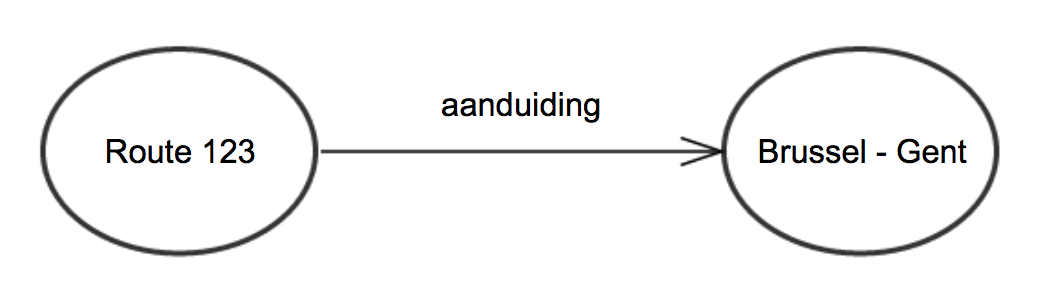
\includegraphics[width=0.5\textwidth]{rdf.png}
\caption{RDF representatie van een triple}
\end{figure}

Een RDF model is dus een gerichte graaf waarbij de knopen en verbindingen benoemd zijn. Er ontstaat als het ware een web van verschillende concepten die met elkaar verweven worden. Data die op zo'n manier opgebouwd is, wordt \textit{Linked Data} genoemd. Om in de praktijk te kunnen refereren naar bepaalde bronnen, zal er identificatie van concepten nodig zijn.

\subsection{Bronidentificatie}
\label{subsec:uri}
Met RDF hebben we een model om bronnen met elkaar te linken en zo feiten te cre\"eren. Om geen verwarring tussen verschillende bronnen te hebben, wordt er gebruik gemaakt van HTTP Universal Resource Identifiers (URI) op het web. Dit heeft dezelfde structuur als een Universal Resource Locator (URL) die in de adresbalk van een browser ingegeven wordt. URI's worden gebruikt om te identificeren, terwijl URL's gebruikt worden om documenten te localiseren. Het kan dus zijn dat een URI een URL is als deze naast identificeren ook gebruikt wordt om meer informatie over te vinden. Het opzoeken van meer informatie over een bepaald onderwerp noemt men \textit{derefereren}.
Neem nu een boek met als IBCN nummer 123 uit een bibliotheek, deze kan ge\"identificeerd worden via \textit{https://bibliotheek.org/books/123}. Als andere bronnen, zoals de auteur, informatie bevatten over dit boek, dan kan er zonder verwarring verwezen worden hiernaar.

Net zoals je bij object geori�nteerd programmeren worden er klasses met bepaalde attributen gemaakt om concepten uit de echte wereld zo re\"eel mogelijk weer te geven. In de wereld van het semantisch web wordt hiervoor gebruik gemaakt van vocabularia.

\subsection{Vocabularium}
Een vocabularium/ontologie is een verzameling klasses en eigenschappen die binnen een bepaalde context samenhoren. Zo is RDF zelf ook een vocabularium waarbij bronnen ofwel een subject, predikaat of object voorstellen. Op dit niveau horen alle bronnen simpelweg tot dezelfde context van triples. Om zaken uit de echte wereld samen te steken, zijn er twee vocabularia die daarbij kunnen helpen: Resource Description Framework Schema (RDFS) en Web Ontology Language (OWL). Met deze vocabularia worden er extra elementen ge�ntroduceerd waarmee er gespecificeerd kan worden of een bron een klasse, eigenschap, waarde of datatype voorstelt. 

Zo werd er voor GTFS data ook een vocabularium\footnote{vocab.gtfs.org/terms} opgesteld. Als we dit toepassen op het voorbeeld van daarnet, zien we dat een triple wordt voorgesteld door 2 URI's en een waarde voor het object.

\begin{figure}[h!]
\centering
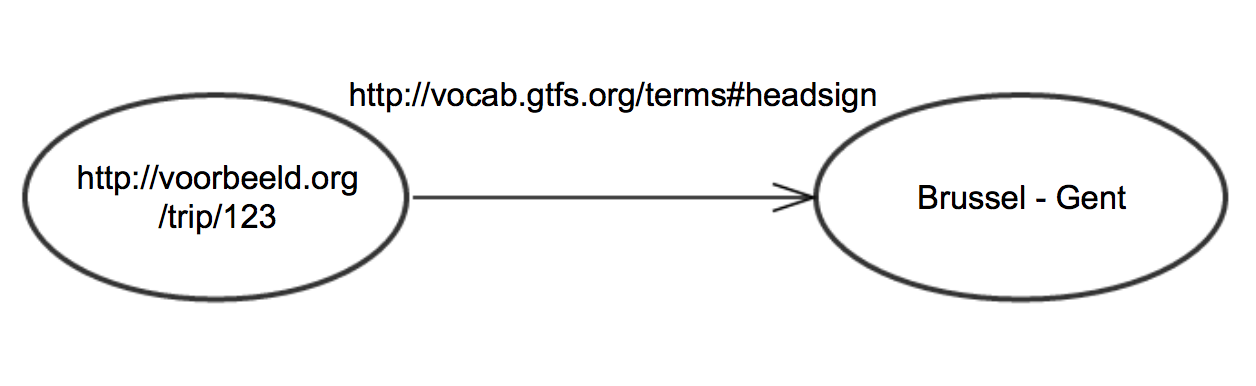
\includegraphics[width=0.5\textwidth]{rdfvocab.png}
\caption{Triple met URI's}
\end{figure}

Om een toepassing te kunnen bouwen wordt data in een bepaald formaat gegoten. Extensible Markup Language (XML) en JavaScript Object Notation (JSON) zijn meest bekende voor webapplicaties te bouwen. Voor beiden is er een uitbreiding voor Linked Data gemaakt: RDF/XML en JSON-LD. Doordat JSON als standaard dataformaat op het web beschouwd wordt zullen we enkel dieper ingaan op JSON-LD.

%\subsection{Re\"ificatie}
%
%%Om niet telkens de volledige URI te moeten typen wordt er gebruik gemaakt van prefixen. Volgende prefix wordt gebruikt in de voorbeelden:
%%PREFIX vb: <http://voorbeeld\#>
%
%Nu dat we een collectie triples hebben, willen we meer informatie over bepaalde triples zelf. (Is het mogelijk om alle triples met bepaald subject of subject+predikaat te re\"ificeren?) Om dit te kunnen doen wordt de triple in zijn geheel als bron behandeld. Dit proces wordt re�ficatie genoemd.
%Stel, we hebben volgende triple: subject: ?ex:trein123?, predikaat: ?ex:isGestationeerdIn?, object: ?ex:Rijsel?. Voor een transportbedrijf kan het handig zijn om te weten welke conducteur de trein heeft gestationeerd. Om deze informatie toe te voegen aan de triple, wordt er een subject gemaakt met als type rdf:statement:
%
%\begin{lstlisting}[label=reificatie,caption=Re\"ificatie van een triple]
%ex:treinStationering1            rdf:type    rdf:statement
%ex:treinStationering1            rdf:subject    ex:trein123
%ex:treinStationering1            rdf:predicate    ex:isGestationeerdIn
%ex:treinStationering1            rdf:object    stations:Rijsel
%ex:treinStationering1        rdf:conducteur    conducteurs:1
%\end{lstlisting}
%
%Nu hebben we een attribuut toegevoegd over onze oorspronkelijke triple. Wat we willen is een context toevoegen aan een collectie triples. Een context wordt net als een andere bron ge�dentificeerd met een URI. Deze wordt simpelweg als attribuut toegevoegd aan de triples.
%
%Dit zorgt uiteraard voor onnodig veel extra triples:
%
%TO = aantal originele triples
%TN = aantal nieuwe triples
%$\rightarrow$ TN = 3 x TO + 1
%

\subsection{JSON-LD}

Als je de openingsuren van een winkel opzoekt in een zoekmachine, gebeurt het vaak dat je een overzicht met informatie bekomt zonder te moeten verderklikken naar een website. Meestal wordt er gebruik gemaakt van JSON-LD om deze informatie aan zoekmachines duidelijk te maken.
JSON-LinkedData is dus een serialisatie formaat voor gelinkte data. Het grote voordeel van JSON-LD is de compabiliteit met bestaande tools die met JSON werken. Zo kan een JSON-LD document als apart script bestand toegevoegd worden aan een website om semantische informatie weer te geven. 
Een JSON-LD document bestaat uit twee delen: een context die bepaalt hoe de data ge\"interpreteerd moet worden en de data zelf. Listing\ref{routejson} bevat informatie over het route voorbeeld in JSON.

\begin{lstlisting}[label=routejson,caption=Voorbeeld trip in JSON.]
{
	"trip id": "trip 123",
	"aanduiding": "Brussel - Gent"
}
\end{lstlisting}

Om deze informatie semantisch te beschrijven, wordt er context toegevoegd. In listing \ref{tripjsonld}  gebruiken we als context de Linked GTFS ontologie. Het type 'trip' wordt toegevoegd met het sleutelwoord '@type'. Er is ook een \textit{prefix} 'trip:' toegevoegd om de leesbaarheid te verhogen. Het is een goede gewoonte om elke bron een eigen identificering geven met behulp van '@id'.

\begin{lstlisting}[label=tripjsonld,caption=Voorbeeld trip in JSON-LD.]
{
	"@context": "http://vocab.gtfs.org/terms",
	"@type": "Trip",
	"trip": "http://voorbeeld.org/trips/",
	"@id": "trip:123",
	"shortName": "trip 123",
	"headsign": "Brussel - Gent"
}
\end{lstlisting}

Dit JSON(-LD) object bevat nu enkel informatie over de entiteit 'trip:123'. Als er meerdere trips zijn met dezelfde context is het handiger om gebruik te maken van benoemde grafen (Engels: \textit{Named Graphs}).

\subsection{Benoemde grafen}

Triples kunnen onderverdeeld worden in grafen. Dit is handig om eigenschappen, metadata... toe te kennen aan een groep triples. In hoofdstuk \ref{subsec:hypermedia} zal blijken dat dit voor hypermedia API's een belangrijke rol speelt. De oorspronkelijke triple is nu een quad geworden met \textit{\textless graaf\textgreater \textless subject\textgreater \textless predikaat \textgreater \textless object\textgreater}. Een voorwaarde is dat de graaf zelf ook ge\"identificeerd wordt met een URI zodat er van buitenaf hiernaar gerefereerd kan worden.

In JSON-LD wordt er gebruik gemaakt van het sleutelwoord '@graph' waarin een array van alle entiteiten van een graaf komt. Listing \ref{tripjsonldgraph} toont hoe makkelijk het is om metadata toe te voegen aan de graaf.

\begin{lstlisting}[label=tripjsonldgraph,caption=Voorbeeld trip in JSON-LD met benoemde graaf.]
{
	"@context": "http://vocab.gtfs.org/terms",
	"dc": "http://purl.org/dc/terms/",
	"dc:publisher": "Brecht Van de Vyvere",
	"@id": "http://voorbeeld.org/graaf/1",
	"@graph":
	[
		{
			"@id": "trip:123",
			"@type": "Trip",
			"trip": "http://voorbeeld.org/trips/",
			"shortName": "trip 123",
			"headsign": "Brussel - Gent"
		}, ...
	]
}
\end{lstlisting}

JSON-LD data kan omgezet worden naar triples om die dan vervolgens in te laden in een triplestore. Hierop kunnen dan vragen afgevuurd worden om informatie te bekomen.

\subsection{SPARQL}
\label{sparql}
SPARQL Protocol and RDF Query Language (SPARQL) is een zoektaal specifiek voor data in RDF formaat. Hiermee kan gelijk welke vraag gesteld worden aan een \textit{triplestore}. In lijst \ref{vbsparqlquery} zie je een voorbeeld SPARQL-query die de URI's van alle verschillende luchthavens in Itali\"e opvraagt.

\begin{lstlisting}[label=vbsparqlquery,caption=Voorbeeld van een SPARQL query.,firstnumber=1]
"SELECT DISTINCT ?entity 
WHERE {
	?entity a dbpedia-owl:Airport;
			dbpprop:cityServed dbpedia:Italy.
}"
\end{lstlisting}

Dit is nu nog een relatief simpele vraag voor een SPARQL-\textit{endpoint}. Het grote probleem \cite{verborgh_ldow_2014} van deze endpoints is dat slechts 30\% effectief 99\% online blijft in een maand. Er is namelijk geen restrictie op het soort queries die uitgevoerd kunnen worden. Voor re\"eele toepassingen is dit ontoelaatbaar dat wanneer veel cli\"ents complexe queries afvuren, de server kan uitvallen.

We zullen eerst het spectrum van \textit{Linked Data fragments} (LDF's) bespreken. Daarna bekijken we een oplossing om SPARQL-endpoints schaalbaar te kunnen query'en.

\subsection{Linked Data Fragments}
\label{ldf}
Een Linked Data dataset is een collectie triples die door een iemand wordt vrijgegeven. Meestal zijn we enkel ge\"interesseerd in bepaalde delen van deze collectie, bijvoorbeeld met een SPARQL-query beschik je enkel over de data die hieraan voldoet. Door een URL te derefereren beschik je enkel over informatie die over dit onderwerp gaat. Deze verschillende interfaces hebben gemeen dat ze een bepaald fragment over eenzelfde dataset voorstellen. In figuur \ref{ldf-as-1} zie je de LDF's as.

\begin{figure}[h!]
\centering
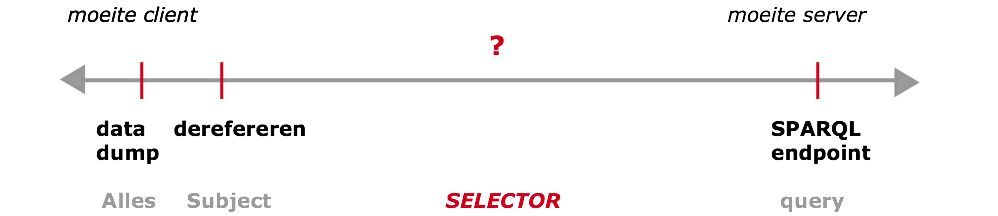
\includegraphics[width=0.8\textwidth]{LDF-as1.png}
\caption{Linked Data Fragments-as}
\label{ldf-as-1}
\end{figure}

Bij elk soort LDF hoort een bepaalde \textit{selector}. Dit is een booleaanse functie die bepaalt of een triple tot het gewenste deel van de dataset behoort of niet. Voor een datadump is deze functie altijd TRUE voor gelijk welke triple. Triples die horen bij een SPARQL-query hebben de query als selector.

Naast data, volgens een bepaalde selector, zijn er nog twee andere eigenschappen die LDF van elkaar onderscheiden:
\begin{itemize}
\item Hypermedia controls. Dit zijn URL's die meer informatie bevatten over bepaalde entiteiten in het fragment, maw informatie over gerelateerde Linked Data Fragmenten. Voor datadumps en het resultaat van een SPARQL query komt dit neer op het derefereren van de URL die een bepaald object voorstelt.
\item Metadata. Dit is informatie over de data zelf, bijvoorbeeld het aantal triples of datum van aanmaak/query'en. Deze informatie wordt in triples toegevoegd aan het datafragment.
\end{itemize}

Het interessante aan deze as is dat verschillende interfaces met elkaar vergeleken kunnen worden. LDF's is dus geen technologie, maar een visie hoe de balans tussen cli\"ent en server kan afgewogen worden. Met data, controls en metadata in het achterhoofd werd in 2014 een oplossing bedacht om Linked Data query'en schaalbaar te maken op het web \ref{tpf}.

\subsection{Triple Pattern Fragments}
\label{tpf}
Bij SPARQL-endpoints (\ref{sparql}) is er een probleem dat endpoints niet 100\% online blijven doordat er geen beperking is in de grootte en complexiteit van queries. Een Triple Pattern Fragments (TPF) is een nieuwe Linked Data Fragment's visie die de trade-off tussen cli\"ent en server afweegt (\ref{ldf-as1b}) door een gulden middenweg te vinden.

\begin{figure}[h!]
\centering
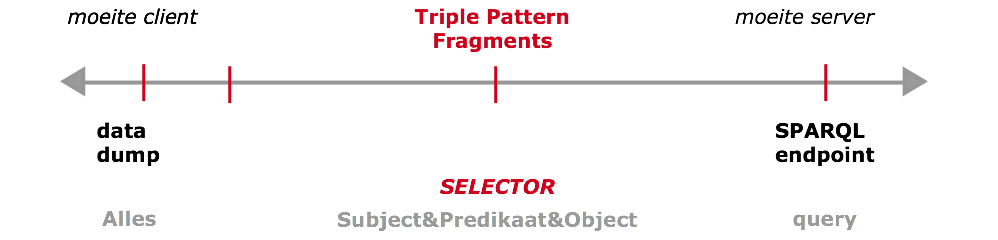
\includegraphics[width=0.8\textwidth]{LDF-as1b.png}
\caption{Linked Data Fragments-as met Triple Pattern Fragments.}
\label{ldf-as1b}
\end{figure}

Deze gulden middenweg houdt twee zaken in:
\begin{itemize}
\item servers bieden een simpele, \textit{low-cost} interface aan.
\item cli\"ents zijn verantwoordelijk voor het oplossen van bepaalde queries. 
\end{itemize}

\subsubsection{Server}
De server is verantwoordelijk voor het teruggeven van triples die voldoen aan een bepaald triple patroon. Zo'n patroon is de combinatie van een subject, predikaat en object waarvan minstens een element een waarde heeft. Een voorbeeld van HTTP template van een TPF-server is te zien in lijst \ref{tpf-interface}. Dankzij hypermedia controls is het mogelijk om een LDF gepagineerd terug te geven. Dit wordt gedaan met behulp van de Hydra hypermedia vocabularium\footnote{http://www.w3.org/ns/hydra/core\#}: hydra:totalItems, hydra:itemsPerPage, hydra:firstPage, hydra : nextPage. Bij \ref{tpf-client} zal het totaal aantal items z'n nut bewijzen.

\begin{lstlisting}[label=tpf-interface,caption=Triple Pattern Fragments interface]
http://triplepatternfragments.org?subject={...}&predikaat={...}&object={...}
\end{lstlisting}

Het berekenen van triples die aan zo'n patroon voldoen is relatief simpel voor een server. Dankzij het beperkt aantal parameters kan er aan HTTP caching gedaan worden. Hierdoor is het mogelijk om veel cli\"ents tegelijk aan te kunnen en is het probleem van SPARQL-endpoints aan de kant geschoven.

\subsubsection{Client}
\label{tpf-client}
Bij SPARQL kon de client gelijk welke vraag stellen aan de server en kreeg daar (hopelijk) antwoord op. Nu is de client verantwoordelijk voor het oplossen van een query door de meerdere simpele vragen te stellen aan de server. Dit gaat ten koste van bandbreedte.

Om het algoritme uit te leggen, gebruiken we het voorbeeld met Italiaanse luchthavens van \ref{vbsparqlquery}. De WHERE-clausule bestaat uit triple patronen: de eerste stelt LDF voor van alle luchthavens en het tweede patroon stelt alle entiteiten die ten dienste van Itali\"e staan. De eerste stap van het algoritme haalt voor beide patronen het eerste fragment op. Dankzij metadata weet de cli\"ent welk patroon het minste triples bevat. Over het resultaat van dit patroon wordt er ge\"iterereerd en worden de variabelen hiervan ingevuld bij de andere WHERE-clausules. Nu wordt hetzelfde algoritme recursief uitgevoerd op de ingevulde, overgebleven WHERE-clausules. Als er in het voorbeeld 1000 luchthavens zijn (eerste patroon), maar slechts 10 entiteiten zijn die Itali\"e dienen (tweede patroon) dan wordt het tweede patroon als startpatroon gekozen. Vervolgens wordt elke triple van dit patroon \textit{gejoint} met het tweede patroon. Als de \textit{count} metadata van deze join een is, weten we dat dit een goed antwoord is.

Zoals je kan zien is TPF een \textit{greedy} algoritme doordat telkens het kleinste LDF van een bepaald patroon gekozen wordt. Een van de voordelen van deze manier van werken is dat het resultaat \textit{gestreamt} kan worden. In tegenstelling tot SPARQL hoeft de cli\"ent niet te wachten op het volledige resultaat om resultaten te tonen aan de gebruiker.

\subsection{Analogie met routeplanning}
Een SPARQL-endpoint is vergelijkbaar met een routeplanner API: een server staat in voor het berekenen van een oplossing op een complex vraag. Een cli\"ent kan bepaalde vragen stellen aan een server. Deze laatste berekent oplossingen en stuurt deze terug. Een SPARQL-server vraagt als input een query, terwijl een routeplanningserver complexe queries probeert op te lossen via een interface met HTTP parameters. Beiden problemen kunnen opgelost worden door de intelligentie te verschuiven van de server naar de cli\"ent en ervoor te zorgen dat de server een simpele, cachebare interface aanbiedt.
Waar Triple Pattern Fragments (TPF) een oplossing biedt voor het query'en van RDF triples op het web, zal later (hoofdstuk \ref{lc}) aangetoond worden hoe dit succesverhaal toegepast kan worden voor routeplannen via Linked Connections (LC). 

In volgende sectie bespreken we enkele richtlijnen voor het bouwen van duurzame Web API's.

\section{REST}

REST staat voor Representational State Transfer. Dit is een set van beperkingen om een architectuur te bekomen die makkelijk uitbreidbaar en gedistribueerd is. Wanneer een Web API aan alle beperkingen voldoet, is deze \textit{RESTful}. Hieronder volgt een overzicht van deze beperkingen.

\subsection{Beperkingen}
\begin{itemize}
\item Client-server: een client en server moeten losgekoppeld zijn. De server biedt voor een uniforme interface aan dat door verschillende soorten cli\"ents (app's, websites...) gebruikt kan worden.
\item Staatloos: de server houdt geen staat bij van de client. Als twee requests R1 en R2 dezelfde informatie opvragen, moet R2 hetzelfde antwoord krijgen als R1. De informatie die de server van de cli\"ent krijgt zou voldoende moeten zijn om een antwoord terug te kunnen geven.
\item Cachebaar: antwoorden van de server moeten gecachet worden. Als twee dezelfde aanvragen worden verstuurd, mag enkel de eerste effectief berekend worden\footnote{Rekening houdend met de ingestelde cacheregels die bijhouden hoelang bepaalde document gecachet mogen worden.}. De tweede aanvraag krijgt als het ware een kopie van de eerste. Dit heeft als voordeel dat de client sneller antwoordt krijgt en dat de server geen dubbel werk moet doen.
\item  Gelaagd systeem: een server bestaat uit verschillende lagen om zo modulair mogelijk te zijn. Hierdoor is het mogelijk om bepaalde functionaliteiten te verspreiden over verschillende servers om overbelasting te vermijden.
\end{itemize}

Om een uniforme interface te kunnen aanbieden, moet de server rekening houden met een aantal bijkomende beperkingen:
\begin{itemize}
\item Resources: niet enkel elke bron moet identificeerbaar (zie ook  \ref{subsec:uri}) zijn met een onveranderlijke URI, maar ook elke collectie. Een URI van een bron bestaat uit de URI van de collectie waartoe het behoort + '/' + de identificatie van de bron zelf.
\begin{lstlisting}[label=restcollectie,caption=Een REST collectie 'boeken' bevat een boek met als identificatie 1.]
'http://voorbeeld.org/boeken/1'. 
\end{lstlisting}
Er kunnen meerdere representaties van zo'n bron of collectie zijn: HMTL, JSON-LD, XML, Turtle... Met behulp van \textit{content negotiation} kan het gewenste formaat verkregen worden.
\item Acties: Om Create/Read/Update/Delete (CRUD) operaties toe te passen op zo'n resource wordt er gebruik gemaakt van volgende HTTP methodes: GET, POST, PUT, DELETE. Complexere acties, zoals sharen, filteren etc., bestaan meestal uit een werkwoord die de actie omschrijft. Om bronidentificatie niet te ondermijnen wordt dit werkwoord na de bron URI met een '?' geplaatst. Listing \ref{complexeactie} toont een voorbeeld van zo'n complexe actie.
\begin{lstlisting}[label=complexeactie,caption=Zoek-actie op een bron.]
http://voorbeeld.org/trips?zoek="Brussel - Gent"
\end{lstlisting}
\item Hypermedia: \label{subsec:hypermedia} Om de interface van een API uniform te maken, is een van de beperkingen die opgelegd wordt \textit{Hypermedia as the Engine of Application State}, kortweg HATEOAS. Hypermedia is simpelweg het volgen van links. Een Hypertext Markup Language (HTML) document zit vol met links naar foto's, video's, andere pagina's etc. HTML toont welke acties mogelijk zijn en als mens bepalen we zelf waar we ge\"interesseerd in zijn. Met dit idee in gedachte zijn Hypermedia API's ontworpen. Zo'n API geeft mee aan de cli\"ent welke acties allemaal mogelijk zijn en dan is het aan de cli\"ent om hier slim mee om te gaan. Deze functionaliteit wordt beschreven in een semantisch formaat zoals JSON-LD. Net zoals een website aangepast kan worden zonder dat de boodschap verloren gaat, kan een Hypermedia API aangepast worden zonder dat de cli\"ent hierbij geherprogrammeerd moet worden.
\end{itemize}

\section{Routeplanning algoritmen}

\subsection{Dijkstra}

\subsection{Heuristieken}

\subsection{CSA}
\label{csa}

\subsubsection{Alternatieve wegen}

\subsubsection{Realtime informatie}

\section{Bestaande routeplanners}

\subsection{Transitland}

\subsubsection{OneStop-ID's}

\subsection{Navitia}




\chapter{Linked Connections}
\label{lc}

Linked Connections \cite{colpaert_iswc_2015} is een framework die \textit{client-side} routeplanning mogelijk maakt. Volgende sectie verduidelijkt hoe de huidige implementatie werkt. Vervolgens wordt uitgelegd hoe connecties worden gegenereerd uit een GTFS feed. Ten slotte wordt verduidelijkt hoe intermodaal routeplannen werkt.

\section{Principe}

Stel je voor dat je de tram moet nemen naar je werk: je stapt ergens op, wacht vijf stophaltes en aan de zesde stophalte stap je af. Dit is een route die uit zes connecties bestaat. Een connectie is de verbinding tussen een vertrek- en eindstop zonder onderbreking. Bij zo'n connectie horen respectievelijk ook een vertrek- en aankomsttijd. Een route kan berekend worden met het CSA algoritme (zie \ref{csa}) die een query en een gesorteerde lijst op vertrektijd als inputwaarde vereist.

Een Linked Connections server presenteert deze gesorteerde connecties in de vorm van Linked Data Fragments (\ref{ldf}) aan de cli\"ent. Momenteel is het enkel mogelijk om de vertrektijd van een query mee te geven als parameter. Met behulp van texttit{hydra:nextPage} links kan de cli\"ent makkelijk opeenvolgende fragmenten ophalen. (zie figuur \ref{lcfragmenten}).

\begin{figure}[h!]
\centering
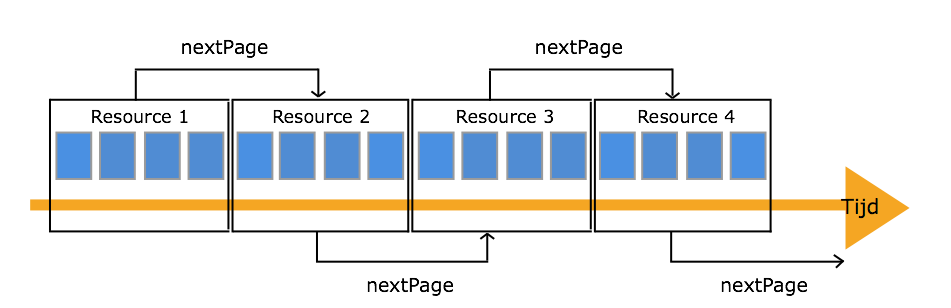
\includegraphics[width=0.8\textwidth]{hypermediafragmenten.png}
\caption{Connecties zijn gesorteerd onderverdeeld in fragmenten die verbonden zijn met hydra:nextPage links.}
\label{lcfragm}
\end{figure}

\begin{lstlisting}[label=queryconnecties,caption=HTTP URL van fragment met Linked Connections.]
http://voorbeeld.org/connecties?vertrekTijd=2015-10-21T11\%3A30
\end{lstlisting}

Het publiceren van de data gebeurt met behulp van drie technologi\"een: 
\begin{itemize}
\item REST zorgt ervoor dat resources cachebaar zijn. Hier zijn fragmenten de resources. Het aantal mogelijke URI's is afhankelijk van het tijdsinterval van de fragmenten. Als T het tijdsinterval in minuten is van de fragmenten, dan kan het aantal mogelijke URI's berekend worden met formule \ref{lc:aantalurisoorspronkelijk}.
\begin{equation} \label{lc:aantalurisoorspronkelijk}
24 * 60 / T
\end{equation}

Als T = 10 min, dan zijn er 144 verschillende fragmenten. De meeste ov-bedrijven rijden niet 24/24 dus in praktijk zijn er nog minder fragmenten. Met behulp van HTTP omleidingen kan dit opgelost worden.
\item Hypermedia zorgt niet enkel voor het vinden van volgende fragmenten, maar ook voor het makkelijk uitbreiden van connecties. Dit kan gaan van een koppeling met geonames tot koffiebars in de buurt.
\item Het semantisch web zorgt voor de semantische interoperabiliteit van de connecties en de API. Dit laat toe om generische clients te bouwen.
\end{itemize}

Op de LDF-as (zie \ref{ldf-lc5}) staat huidige implementatie aan de linkerkant. Het kost de server weinig moeite om data te publiceren door de hoge cachebaarheid. Een cli\"ent moet daarentegen veel connecties scannen om tot een route te komen. Later (\ref{resultaat-origineel}) zal de exacte performantie verduidelijkt worden.

\begin{figure}[h!]
\centering
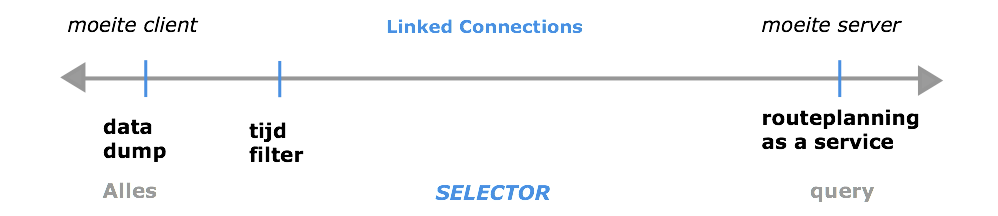
\includegraphics[width=0.8\textwidth]{LDF-as5.png}
\caption{Linked Data Fragmenten-as met Linked Connections}
\label{ldf-lc5}
\end{figure}

\section{Voorbewerking}

Gelinkte connecties worden berekend uit een GTFS \textit{feed}. De convertor in deze masterproef maakt gebruik van een MySQL-databank om queries op uit te voeren. \footnote{Ondertussen is een veel snellere convertor gemaakt die volgens een ander principe werkt, zonder databank. Zie github.com/linkedconnections/gtfs2lc} Het is belangrijk op te merken dat connecties niet gesorteerd moeten zijn bij het voorbewerken. Deze worden later in de databank van de Linked Connections server ingeladen die zelf sorteert. Figuur \ref{inladengtfs} toont een overzicht van de verschillende stappen om connecties te genereren.

\begin{figure}[h!]
\centering
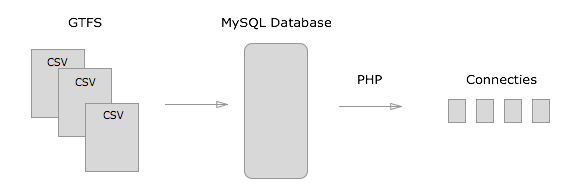
\includegraphics[width=1.0\textwidth]{Preprocessor.png}
\caption{Overzicht hoe connecties worden gegenereerd uit een GTFS feed. Deze wordt ingeladen in een MySQL databank. Met de scripttaal PHP worden connecties gegenereerd hieruit.}
\label{inladengtfs}
\end{figure}

Connecties worden dag per dag berekend. Ofwel worden start- en einddatum meegegeven als parameters, ofwel worden start- en einddatum van de GTFS feed zelf genomen. Vervolgens worden alle services uit \textit{calendar} en \textit{calendar\_dates} van een bepaalde dag opgehaald. Bij elke service hoort een bepaalde \textit{route} en een verzameling \textit{trips} die dan worden opgehaald uit \textit{trips}.
Een laatste stap is het overlopen van \textit{stoptimes.txt}. Uit de combinatie van twee opeenvolgende stoptimes kan een connectie berekend worden. Lijst \ref{vbstoptimes} bevat een voorbeeld van twee opeenvolgende stoptijden van een bepaalde trip.

\begin{lstlisting}[label=vbstoptimes,caption=Vereenvoudigde stoptimes in CSV.]
trip_id,arrival_time,departure_time,stop_id,stop_sequence
16,07:18:00,07:18:00,8200100,1
16,07:33:00,07:33:00,8200110,2
\end{lstlisting}

\begin{figure}[h!]
\centering
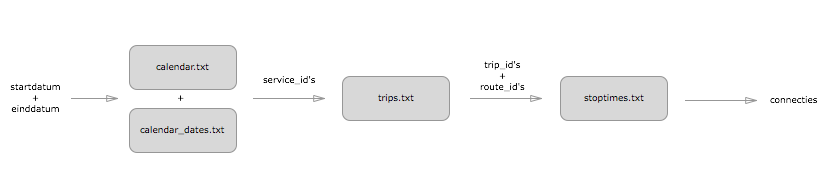
\includegraphics[width=0.8\textwidth]{volgordeconvertor.png}
\caption{Per dag worden de corresponderende service ID's, trip ID's en route ID's berekend. De vertrek-/aankomststopplaats met respectievelijk vertrek-/aankomsttijd worden berekend uit een verzameling stoptimes. }
\end{figure}

Codevoorbeeld \ref{connectiejsonld} toont hoe een connectie eruit ziet bij output. Merk op dat een '@context' niet is toegevoegd en ook niet in een graaf zit. In subsectie \ref{jsonldstream} wordt hierover meer uitleg gegeven.

\begin{lstlisting}[label=connectiejsonld,caption=Connectie voor een bepaalde trip met bijkomstige route in JSON-LD.]
{	
	"@id": "http://example.org/connections/1"
	"@type": "http://semweb.mmlab.be/ns/linkedconnections#Connection",
	"http://vocab.gtfs.org/terms#trip": "16",
	"http://vocab.gtfs.org/terms#route": "route-1",
	"http://semweb.mmlab.be/ns/linkedconnections#departureTime": "2015-10-21T06:18:00.000Z",
	"http://semweb.mmlab.be/ns/linkedconnections#departureStop": "8200100",
	"http://semweb.mmlab.be/ns/linkedconnections#arrivalTime": "2015-10-21T06:33:00.000Z",
	"http://semweb.mmlab.be/ns/linkedconnections#arrivalStop": "8200110"
}
\end{lstlisting}

De tijdszone van vertrek- een aankomsttijd staat in Coordinated Universal Time (UTC). Er moet altijd rekening gehouden worden met de tijdszone van de GTFS feed. In dit voorbeeld \ref{vbstoptimes} werd een feed uit Belgi\"e genomen. Om de Belgische tijd (UTC+1) om te zetten naar UTC moet er een uur afgetrokken worden van de tijd die vermeld staat in GTFS stoptijden.

Een van de moeilijkheden voor het genereren van connecties was het ophalen van trips die voor middernacht vertrekken, en dus geclassificeerd zijn onder die dag, maar na middernacht pas stoppen. GTFS lost dit op door de tijd na middernacht door te tellen, bijvoorbeeld 2u 's nachts staat weergegeven als 26u. Volgens GTFS rijden deze stoptimes allemaal op dezelfde dag, maar voor Linked Connections zijn dit effectief twee verschillende dagen, omdat er met exacte tijden gewerkt wordt.
Om dit op te lossen worden er twee extra vlaggen toegevoegd in de databank of de vertrek- en aankomsttijd van een stoptijd voor of na middernacht plaatsvinden.

Een databank gebruiken heeft als grote nadeel dat de data ingeladen moet worden vooraleer berekeningen kunnen plaatsvinden. In \ref{table:inladengtfs} staat een overzicht van de drie gebruikte datasets in deze masterproef met de tijd om in te laden. Voor zeer grote datasets, zoals De Lijn, is inladen een bottleneck.

\begin{table}[htbp]
\centering
\begin{tabular}{ | l || c | c | c |}
  \hline			
    & Tijd (min) & Grootte (MB) & Periode (weken) \\ \hline
  NMBS & 3.1 & 1.1 & 12  \\
  NS & 8.35 & 21.4 & 56 \\
  De Lijn & 100 & 44 & 10 \\
  \hline  
\end{tabular}
\caption{Tijd om een GTFS feed in te laden in een MySQL databank.}
\label{table:inladengtfs}
\end{table}

Het genereren van connecties zelf gaat een stuk rapper. In \ref{table:connectiesgenereren} zie je dat voor kleine datasets (zoals NMBS en NS) het minder dan minuut duurt om de connecties voor een dag te berekenen. De Lijn scoort opnieuw zeer slecht door de grootte van de dataset.

\begin{table}[htbp]
\centering
\begin{tabular}{ | l || c | c | c |}
  \hline			
    & Tijd (min) & Connecties \\ \hline
  NMBS & 0.21 & 55479 \\
  NS &  &  \\
  De Lijn & 14.97 & 1049186 \\
  \hline  
\end{tabular}
\caption{Tijd om connecties te genereren voor een dag.}
\label{table:connectiesgenereren}
\end{table}

\subsection {JSON-LD stream}
\label{jsonldstream}
Om de connecties als Linked Data te publiceren werd er voor gekozen om JSON-LD te gebruiken. JSON wordt beschouwt als het \textit{de facto} standaardformaat op het web dankzij de compactheid, leesbaarheid en vele handige tools die hiervan gebruik maken. Wanneer een verzameling objecten dezelfde context heeft, zijn er twee mogelijkheden om deze te publiceren:
\begin{itemize}
\item een gemeenschappelijke context voorzien en alle objecten in bijhorende graaf steken (zie \ref{tripjsonldgraph}). Deze methode vereist dat de graaf in het geheugen geladen moet worden vooraleer verdere operaties mogelijk zijn.
\item elk object een context geven (zie \ref{tripjsonld}). Met deze methode kan object per object gestreamt worden, maar zorgt voor grote overhead door de context die telkens mee gepubliceerd wordt.
\end{itemize}
Een oplossing hiervoor is de JSON-LD streamspecificatie \footnote{https://github.com/pietercolpaert/jsonld-stream}. Deze geeft aan dat de context van een object met '@context' van toepassing is op alle andere objecten van het document. Zo moet er maar eenmalig een context opgegeven worden en wordt impliciet verondersteld dat de andere objecten deze context gebruiken.
De voorbewerker kan nu connecties als Linked Data wegschrijven zonder extra dataverlies en gestroomlijnd. Dit stroomlijnen is belangrijk om de data later lijn per lijn te kunnen inladen in een databank.

\section{Client}

De client is verantwoordelijk voor het berekenen van de snelste route. Deze kan met een paar lijntjes code aangemaakt worden (zie \ref{clientvb}).
\begin{lstlisting}[label=clientvb,caption=Code om client op te zetten in JavaScript.]
var planner = new window.lc.Client({"entrypoints" : ["http://example.linkedconnections.org/"]});
planner.query({
			"departureStop": "Brussel-Zuid",
			"arrivalStop": "Gent-Sint-Pieters",
			"departureTime": new Date("2015-11-05T10:00")
			}, function (stream) {
				stream.on('result', function (pad) {
					// pad bevat verzameling connecties die snelste route voorstellen
				});
			 	stream.on('data', function (connectie) {
			 		// connectie is gebruikt geweest voor minimale overspannende boom
			 	});
});
\end{lstlisting}
\label{vbclient}

Linked Connections van verschillende ov-bedrijven worden gedistribueerd opgesteld. De cli\"ent is verantwoordelijk voor het samenvoegen van connecties. In figuur \ref{overzichtclientserver} staat een overzicht van een client - meerdere servers opstelling. Rechts staan twee Linked Connection servers, de ene verantwoordelijk voor de connecties van een vervoersmaatschappij van bussen, de andere van treinen. Links staat een client die de fragmenten ophaalt van beide servers. Voor het scannen zelf kan plaatsvinden, moeten deze samengevoegd worden. Daarna kan de snelste route met Connection Scan Algorithm (CSA) gepland worden.

\begin{figure}[h!]
\centering
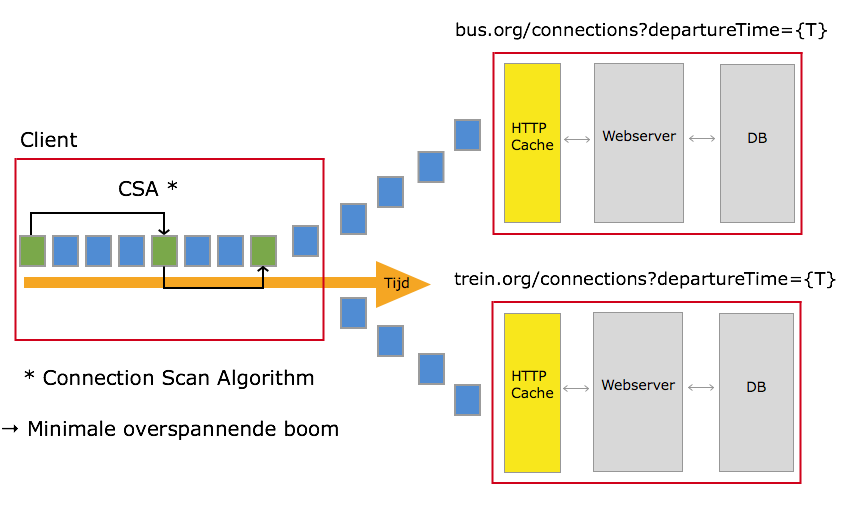
\includegraphics[width=0.5\textwidth]{OverzichtClientServer.png}
\label{overzichtclientserver}
\caption{Opstelling van een client en twee Linked Connections servers.}
\end{figure}

\subsection{Merger}

Een merger voegt meerdere stromen van gesorteerde connecties samen tot een stroom. Dit is noodzakelijk voor de cli\"ent om CSA te kunnen toepassen.

Connecties komen onder de vorm van een \textit{stream} binnen. Zo'n stream werkt asynchroon met events. Deze worden opgeworpen wanneer bijvoorbeeld data beschikbaar is. Figuur \ref{merger} toont een overzicht van een merger. Deze luistert (1) naar de verschillende datastromen tot deze data vrijgeven. De connecties worden toegevoegd in wachtrijen. Wachtrijen (2) hebben als voorwaarde dat ze zelf gesorteerd zijn. Datastromen worden telkens gepauzeerd na het opvangen van data. Dit is noodzakelijk om de cli\"ent beslissingstijd te geven. Zo kan er beslist worden om een bepaalde connectiestroom uit te schakelen of toe te voegen. Een andere reden waarom de merger de connectiestromen pauzeert, is het feit dat de wachtrijen minstens een connectie moet bevatten van elke connectiestroom. Wanneer de merger connecties teruggeeft, worden alle connecties van elke wachtrij met dezelfde lokaal minimale vertrektijd teruggegeven. Zo blijven alle wachtrijen synchroon.

\begin{figure}[h!]
\centering
\includegraphics[width=0.5\textwidth]{merger.png}
\caption{Overzicht merger}
\label{merger}
\end{figure}

\begin{lstlisting}[label=vbclient,caption=Voorbeeldcode van een merger. Deze voegt meerdere stromen van connecties samen.]
"var connectionsStreams = [
    [ 'stream1', connectionsReadStream1 ],
    [ 'stream2', connectionsReadStream2 ],
    ...
];

var connectionsReadStream = new csa.MergeStream(connectionsStreams, query.departureTime);"
\end{lstlisting}

\section{Voor- en nadelen}

\begin{itemize}
\item Routeplanning is een dataprobleem geworden. Datapubliceerders zijn verantwoordelijk voor het publiceren van connecties en bijhorende data. Zo kan er makkelijk data toegevoegd worden via hypermedia: \textit{point of interests}, rolstoelvriendelijkheid etc. De cli\"ent bepaalt zelf welke informatie deze wil gebruiken.
\item Connecties zijn makkelijk distribueerbaar over meerdere servers. 
\end{itemize}

\chapter{Optimalisatie}
\label{opt}

De bedoeling van de optimalisatie is het vergroten van het percentage nuttige connecties. Met basis LCF's werd er enkel in de tijd gefilterd waardoor ook connecties van ontoegankelijke stopplaatsen werden teruggeven. De optimalisatietechnieken die in dit hoofdstuk besproken worden, zullen dit probleem proberen oplossen met behulp van geofiltering.

\section{Geofiltering}

Het CSA-algoritme bouwt met de binnenkomende connecties een minimale overspannende boom. Dit kan visueel voorgesteld worden als een cirkel rondom het vertrekpunt van de query. Het idee van geofiltering bij Linked Connections is om enkel connecties gesorteerd in de tijd �n afstand van het vertrekpunt terug te geven. Een extra filter betekent extra HTTP parameter(s).

\subsection{Geoparameter}
Een eerste inspiratie was om connecties onder te verdelen zoals kaarten als Open Street Maps werken. Hierbij wordt er met \textit{tiles} gewerkt. Een \textit{tile} is een rechthoekig stuk van een kaart die op basis van drie parameters kan ge\"identificeerd worden: het x- en y-co\"ordinaat en een \textit{zoomlevel} z. Bij statische data zoals kaarten is dit zeer handig, omdat deze stukjes cachebaar zijn. Bij transportdata moet er ook rekening gehouden worden met tijd, waardoor zo'n systeem niet haalbaar is.

Resources zijn pas cachebaar als er een beperkte set van URL's zijn. Aangezien elke publieke transportmaatschappij een beperkte set stops heeft, wordt er geopteerd om het vertrekpunt van een query toe te voegen als extra HTTP parameter. Listing \ref{nieuwe-interface}) toont deze nieuwe interface. Connecties die in de buurt van de vertrekstop liggen, hebben zeker initieel een grotere kans om gebruikt te worden. In volgende subsectie bespreken we de criteria om connecties terug te geven. 

\begin{lstlisting}[label=interface-optimalisatie,caption=Interface LDF met optimalisatie]
http://example.org?departureTime={...}&departureStop={...}
\label(label:nieuwe-interface)
\end{lstlisting}

\subsection{Criteria}
In eerste instantie moeten we een "straal"-definitie bepalen. Hiervoor zijn er twee mogelijkheden:

\begin{itemize}
\item De straal tussen de vertrekstop en een stop $s$ is het minimaal aantal connecties nodig om deze te bereiken. Een straal van grootte een stemt overeen met stops die met een connectie bereikt kunnen worden. Een straal van grootte twee is een stop waarvoor twee connecties nodig zijn enzovoort. Connecties worden als het ware \textit{gejoint} aan elkaar.
\item Het minimum aantal overstappen (Engels: \textit{transfers}) wordt als straal van een stop genomen. Dit geeft extra interessante mogelijkheden zoals Pareto-optimale routes bepalen op basis van snelste aankomsttijd �n maximaal aantal overstappen. Dit idee wordt ook bij RAPTOR (\ref{raptor}) gebruikt. Voortaan zullen we de letter $K$ gebruiken voor het minimum aantal overstappen.
\end{itemize}

Deze masterproef maakt gebruik van het aantal overstappen. 

Twee nieuwe termen zullen regelmatig gebruikt worden:
\begin{itemize}
\item \textit{direct bereikbare stop}: dit is een stop dat zonder overstappen bereikbaar is vanuit de vertrekstop. In GTFS termen betekent dit dat de snelste route slecht uit een trip kan bestaan.
\item \textit{indirect bereikbare stop}: dit is een stop die minstens K overstappen vereist vanuit de vertrekstop.
\item \textit{buur}: dit is een stop die direct of indirect bereikbaar is.
\end{itemize}

Een andere belangrijke criteria om geoptimaliseerd connecties terug te geven is dat er geen connecties teruggeven mogen worden van buren die theoretisch gezien nog niet bereikbaar zijn. Voor elke buur is een bepaalde \textit{minimale tijd} nodig om deze te bereiken.

Kortom, voor elke stop moet zijn buren bepaald worden samen met informatie over het minimaal aantal overstappen en minimale tijd om deze te bereiken. Hiervoor wordt er een extra voorbewerkingsfase toegevoegd en wordt er een extra \textit{feature} aan het connectiegenerator script toegevoegd.

\subsection{Direct bereikbare stops}

Connecties worden gegenereerd uit een reeks stoptijden van dezelfde trip. Dit is informatie die gebruikt kan worden om direct bereikbare stops te berekenen. Zo'n reeks stelt een aantal paren stops voor met een bepaalde tijd die nodig is in die trip. Tijdens het genereren van connecties wordt voor elke stop een minimale overspannende boom bijgehouden met als knopen rechtstreeks bereikbare stops en als verbindingen de minimale tijd. Nadat de connecties gegenereerd zijn wordt deze informatie weggeschreven naar een CSV-bestand zodat we dit kunnen hergebruiken om buren mee te berekenen.

\subsection{Buren}

Het berekenen van buren houdt het vinden van niet-direct bereikbare stops voor elk stop in. Een indirect bereikbare stop van $s$ met minimum aantal overstappen $K=1$ is een direct bereikbare stop van een direct bereikbare stop van $s$ die niet direct bereikbaar is bij $s$ zelf. Als er $n$ stops zijn in een dataset, moeten er $n*n$ afstanden berekend worden. Dit zou gemakkelijk met Floyd-Warshall kunnen, maar bij grote netwerken zoals bij De Lijn is er een probleem met geheugen. De Lijn heeft namelijk afgerond 35000 stopplaatsen waardoor een matrix van 35000 x 350000 in het geheugen moet gehouden worden. Om dit toch te kunnen berekenen, maken we gebruik van een algoritme die gebaseerd is op Dijkstra. Pseudocode hiervan is te vinden in \ref{mob-stop}. Er kan ingesteld worden tot hoeveel overstappen er verder gezocht moet worden. Het algoritme maakt gebruik van een wachtrij van stops die nog bekeken moeten worden. Elke stap probeert de minimale tijdsafstand en/of aantal overstappen te minimaliseren van een buur van een stop. Het object dat bekomen wordt voor een bepaalde stop staat afgebeeld in listing \ref{serverstopdata}. Dit wordt weggeschreven naar een aparte buren-tabel op een LC server.

\begin{lstlisting}[label=serverstopdata,caption=Data over stop serverside]
{
	stop_id : 123,
	aantal_direct_bereikbare_stops: X,
	// andere metadata over de stop
	buren: [
		{
			stop_id: 253,
			minimaleTijdsAfstand: 1800, // seconden
			K: 2
		}, {
		...
		}
	]
}
\end{lstlisting}

\begin{algorithm}
  \caption{Berekenen van Minimale Overspannende Boom van burenstops voor een GTFS stops.txt. $T$ is het maximaal aantal overstappen waarmee rekening gehouden wordt.}
  \label{mob-stop}
  \begin{algorithmic}
  \State K $\leftarrow$ natuurlijk getal
  \For { elke stop $s$ in stops.txt }
  \Statex // Initialisatie
    \State var mob = \{\};
    \State var wachtrij = []; // nog te bezoeken stops
    \For  {elke direct bereikbare stop $b$ van $s$}
    	\State mob[b.stop\_id] = \{ K : 0, tijdsafstand : b.tijdsafstand,  aantal\_rechtstreekse\_buren: start.buren.length \};
	\If { (T \textgreater 1) } // 
	\State wachtrij.push(b.stop\_id);
	\EndIf
    \EndFor
    
    \While{ (  wachtrij niet leeg is ) }
    	\State var start = wachtrij.shift();
	\For  { elke direct bereikbare stop $b$ van $start$ }
		// Zit nog niet in MOB
		\If{  (!mob[b.stop\_id]) }
		\State mob[b.stop\_id] = \{ K: start.K + 1, tijdsafstand: start.tijdsafstand + b.tijdsafstand, aantal\_rechtstreeks\_buren: start.buren.length \};
			\If { (b.K \textless T) }
				\State wachtrij.push(b); // nog verder te onderzoeken
			\EndIf
		\Else {
			\If { (start.K + 1 \textless  mob[b.stop\_id].K) }
				mob[b.stop\_id].K = start.K + 1;
			\EndIf
			\If { (start.tijdsafstand + b.tijdsafstand \textless  mob[b.stop\_id].tijdsafstandl) }
				mob[b.stop\_id].tijdsafstand = start.tijdsafstand + b.tijdsafstand;
			\EndIf	
		}
		 \EndIf
	\EndFor 
    \EndWhile
    \EndFor
  \end{algorithmic}
\end{algorithm}

Zoals je kan zien in \ref{mob-stop} wordt er ook het aantal rechtstreeks bereikbare stops bijgehouden voor elke buur. Volgende sectie zal hierover meer uitleg geven.
Tabel \ref{table:burenberekenen} toont hoelang het duurt om de buren te berekenen volgens de grootte van het netwerk van de NMBS en NS.

\begin{table}[htbp]
\centering
\begin{tabular}{ | c || c | c | }
  \hline
  Dataset & Aantal stops & Tijd (min) \\ \hline
  NMBS & 597  & 6.35 \\
  NS & 2532 &  21.19 \\
\hline  
\end{tabular}
\caption{Tijd om buren van alle GTFS stops te berekenen.}
\label{table:burenberekenen}
\end{table}

In volgende sectie bespreken we hoe gebruik gemaakt kan worden van deze informatie om het routeplannen sneller te maken.

\section{Neighbour Linked Connections Fragment}

Wanneer de cli\"ent een request met vertrektijd �n vertrekstop opvraagt, geeft de server connecties terug die zowel uit de vertrekstop als uit de buren vertrekken. Zo'n fragment op basis van vertrektijd en vertrekstop noemen we \textit{Neighbour Linked Connections Fragment} (NLCF). Op deze manier kan de cli\"ent veel informatie in een request bekomen. De query die hierbij gebruikt wordt op de server staat vermeld in listing \ref{optimalisatiequery}.
\begin{lstlisting}[label=optimalisatiequery,caption=SQL query template van optimalisatie.]
SELECT *
FROM connecties
WHERE (vertrekStop = queryStop && vertrekTijd > queryTijd && vertrekTijd < queryTijd + interval)
OR (vertrekStop = buur1 && vertrekTijd > vroegste_vertrektijd_buur1 && vertrekTijd < vroegste_vertrektijd_buur1 + interval)
OR (vertrekStop = buur2 && vertrekTijd > vroegste_vertrektijd_buur2 && vertrekTijd < vroegste_vertrektijd_buur2 + interval)
OR ...
\end{lstlisting}

Vooraf moet een bepaald tijdsinterval ingesteld worden waarin de snelste route zich zou moeten bevinden.

\begin{figure}[h!]
\centering
\includegraphics[scale=0.6]{burenconnecties}
\caption{Neighbouring Linked Connections Fragment bevat connecties van vertrekstop en buren binnen een bepaald tijdsinterval.}
\label{burenconnecties}
\end{figure}

Het basisidee is dat een NLCF meer nuttige informatie bevat dan een basic LCF. Hierbij zijn er twee trade-offs:

\begin{itemize}
\item Het maximaal aantal overstappen $K$. Stops die verder liggen hebben een grotere kans op meer overstappen. De vraag is of het nuttig is om moeilijk bereikbare stops in rekening te brengen.
\item Het tijdsinterval $T$ waarin connecties van een stop worden teruggegeven.
\end{itemize}

% Deze parameters zijn dynamisch aanpasbaar.

Een Linked Connections server is nu verantwoordelijk voor beide soorten fragmenten. Volgende sectie bespreekt een eerste mogelijkheid dat de cli\"ent kan opgaan.

\section{Heuristische techniek}
\label{heuristiek-client}

De heuristische techniek maakt enkel gebruik van neighbouring LC Fragments. Als het antwoord niet gevonden is met een request, moet een volgende vertrekstop gekozen worden. Hiervoor wordt er gebruik gemaakt van een heuristiek. Deze bepaalt aan de hand van enkele parameters welke stop het meest kans heeft om op het pad van de snelste route te liggen. De stop met de hoogste score wordt gekozen als vertrekstop van de volgende NLCF.

\subsection{Parameters}
De heuristiek in deze implementatie maakt gebruik van volgende parameters:
\begin{itemize}
\item De snelheid $v$ van de connectie. De afstand $d$ tussen de stop en de eindbestemming, met andere woorden hoe dichter bij onze bestemming hoe beter. Een stop die op de rechtstreekse weg tussen vertrekpunt en eindpunt ligt, krijgt zo een hogere score.
\item De cosinus-gelijkaardigheid. De cosinus van twee vectoren bepaalt hoe sterk de vectoren in dezelfde richting liggen. De ene vector bestaat uit het start- en eindpunt van de connectie en de andere uit start- en eindbestemming van de route. 
\item De belangrijkheid van een station. Als maatstaf kan het aantal rechtstreeks bereikbare stops vanuit een bepaalde stop genomen worden. Het gebeurt vaak dat een snelste route niet de meest rechtstreekse weg is. Dit is vooral het geval bij treinen. Er is bijvoorbeeld een rechtstreekse trein tussen Gent en Lichtervelde, maar vaak is het dat de snelste route via Brugge gaat. Brugge ligt niet op de rechtstreekse weg tussen Gent en Lichtervelde dus moet er metadata zijn die de belangrijkheid van bepaalde stations aanduidt. Er moet een soort van knoophi\"erarchie van stops komen zoals we besproken hebben in de literatuurstudie. In tabel \ref{table:rechtstreeksestops} zie je een overzicht van enkele stations met hun aantal rechtstreekse stops en drukte \footnote{De drukte van een station is bepaald met de open dataset van stations: github.com/irail/stations}. Brussel is het meest centrale punt in Belgi\"e. Zijn rechtstreekse stops zijn dan ook het meest van alle stations en in heeft een gelijke proportie met het gemiddeld aantal stoptijden. Gent en Antwerpen zijn gelijkwaardig in grootte en drukte. Antwerpen heeft met minder rechtstreekse stopplaatsen toch een grotere frequentie. De laatste drie stations bestaan uit twee stations waarlangs verschillende routes samenkomen en een station waar niet overgestapt kan worden. Dit weerspiegelt zich zowel in de eerste als tweede waarde. We kunnen concluderen dat het aantal rechtstreekse stops een goede parameter voor de metaheuristiek is.

\begin{table}[htbp]
\centering
\begin{tabular}{ | l || c | c |}
  \hline			
  Station & Aantal rechtstreekse stops & Gemiddeld aantal stoptijden per dag \\ \hline
  Brussel-Centraal & 350 & 634 \\ 
  Gent-Sint-Pieters & 175 & 309 \\
  Antwerpen-Centraal & 154 & 467 \\
  Deinze & 88 & 44 \\
  Lichtervelde & 77 & 53 \\ 
  Tielt & 39 & 19 \\
  \hline  
\end{tabular}
\caption{Overzicht van enkele stations van de NMBS met hun aantal rechtstreeks bereikbare stops en gemiddeld aantal stoptijden per dag.}
\label{table:rechtstreeksestops}
\end{table}

\end{itemize}

\subsection{Formule}
De metaheuristiek bestaat uit volgende formule:

\[ prioriteit = \alpha * afstand/tijd + \beta * aantal\_rechtstreekse\_stops + \gamma * \cos(theta) \]

\begin{itemize}
\item De snelheid (het quoti\"ent van afstand en tijd van een connectie). Een connectie die in korte tijd een grote afstand aflegt, heeft een grotere kans om tot de snelste route te horen.
\item Het aantal rechtstreekse stops duidt de belangrijkheid van het station aan.
\item De cosinusgelijkheid theta: de cosinus van de hoek tussen de connectievector en de vector van rechtstreekse weg bepaalt de mate of de connectie ons veel dichter bij het doel brengt.
\end{itemize}

Deze parameters moeten eerst genormaliseerd worden zodat elke parameter een score heeft van 0 tot en met 1. Wanneer de cli\"ent een fragment opgehaald heeft, wordt er een bepaald aantal connecties eerst geanalyseerd voor de normalisatie. Voor elke parameter wordt er de maximale waarde bepaald. Daarna wordt deze genormaliseerde waarde vermenigvuldigd met een bepaalde gewichtsfactor alpha, beta.... De sommatie bepaalt de prioriteit van het station. Deze wordt in een prioriteitswachtrij gestopt om in $O(1)$ tijd het belangrijkste station te kunnen opvragen.

Het toepassen van de heuristiek en toevoegen aan de prioriteitswachtrij wordt enkel op nuttige connecties toegepast. Dit wil zeggen dat CSA deze connectie heeft toegevoegd aan de minimale overspannende boom. De module die verantwoordelijk is voor het ophalen van fragment wacht dus tot alle connecties gescant zijn om vervolgens het volgende beste fragment te bepalen.

\subsection{Voordeel}
\begin{itemize}
\item Om niet van 
\end{itemize}

\subsection{Nadelen}
\label{heuristiek-nadelen}
\begin{itemize}
\item Er wordt minder effici\"ent omgegaan met connecties dan gewenst. Een NLCF geeft voor elke  buurstop ($K <= max K$) connecties terug binnen een bepaald tijdsinterval. Dit moet allemaal in een fragment waardoor het tijdsinterval klein moet blijven. Hierdoor daalt de kans dat verre buren bereikt kunnen worden. Wanneer een nieuwe vertrekstop gekozen wordt, kunnen er connecties voor de tweede, derde... keer verzonden worden. Een groot deel van de connecties van een nieuwe vertrekstop zijn ook onnuttig, namelijk deze die geografisch liggen aan de kant van waar vertrokken werd.
\item Het werken met een heuristiek zorgt voor een suboptimale oplossing. Dit wil zeggen dat er een route gevonden wordt, maar niet gegarandeerd de snelste. Dit ligt aan het feit dat een heuristiek niet voldoende is om de snelste route te bepalen. Zo zou er voor elk station een maximale tijdswaarde bepaald moeten worden die ervoor zorgt dat de connectie met de snelste route hierin ligt. Een mogelijke uitbreiding zou zijn om $T$ en $K$ te maximaliseren en dit fragment dan te pagineren. Een grotere $T$ en $K$ zorgt ervoor dat meer queries in een fragment opgelost kunnen worden. Wegens tijdsgebrek om te onderzoeken of een maximale tijdsinterval per stop mogelijk is, gaan we hier niet dieper op in. Er is wel geweten of de snelste route binnen het tijdsinterval $T$ ligt van het eerste NLCF.  
De volgende besproken techniek bouwt verder op dit idee.
\end{itemize}

\section{Speed-up techniek}

De \textit{speed-up} techniek maakt enkel in het begin gebruik van een NLCF. Indien het resultaat nog niet gevonden is, wordt verdergezocht met basic LCF's. Een NCLF heeft een veel grotere effici\"entie (zie \ref{dataverbruik-heuristiek}. Door verder te zoeken met basic LCF's kan de snelste aankomsttijd gegarandeerd worden.

\begin{figure}[h!]
\centering
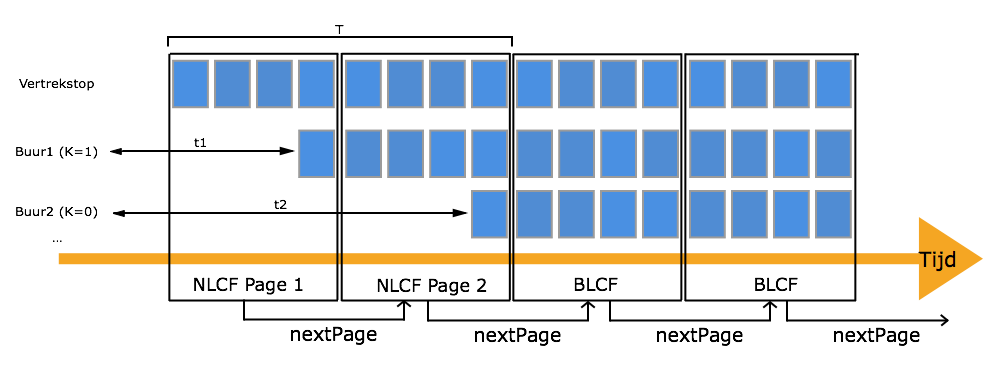
\includegraphics[scale=0.4]{OptimalisatieHypermedia}
\caption{Overzicht van resources van speed-up optimalisatietechniek.}
\label{OptimalisatieHypermedia}
\end{figure}

%Uit de resultaten \ref{dataverbruik-heuristiek} blijkt dat het eerste fragment bepaalt of het resultaat gevonden wordt of niet. Hierbij bevat het eerste fragment drie keer zoveel nuttige connecties.

\subsection{Hypermedia}

De originele implementatie maakt gebruik van hydra:nextPage links om volgende fragmenten te vinden. Dit principe kunnen we toepassen op een NLCF (zie ook \ref{OptimalisatieHypermedia}). Op deze manier kunnen we een grotere $T$ waarde instellen zonder dat kleinere routes onnodig veel connecties downloaden. $K$ moet maximaal zijn om te kunnen garanderen dat de optimale oplossingen ertussen zit.
Uit de resultaten van basic Linked Connections Fragments (zie \ref{fragmentgrootte}) blijkt dat queries gemiddeld het snelst opgelost zijn als de fragmenten een grootte hebben van rond de duizend connecties. Het initi\"ele NLCF wordt per duizend connecties onderverdeeld. Listing \ref{interface-met-hypermedia} toont de nieuwe interface. Het NLCF fragment bevat naast tijdsinterval $T$ ook een pagina-grootte. Hiervoor kan hetzelfde tijdsinterval genomen worden als basic LCF's.

\begin{lstlisting}[label=interface-optimalisatiemethypermedia,caption=Interface optimalisatie met hypermedia links]
http://example.org?departureTime={...}&departureStop={...}&page={...}
\end{lstlisting}
\label{interface-met-hypermedia}

Met deze techniek worden de twee nadelen (\ref{heuristiek-nadelen} van vorige techniek weggewerkt:
\begin{itemize}
\item Er is een hogere effici\"entie, omdat een groter tijdsinterval gekozen kan worden. Daarbij worden connecties slechts een keer teruggeven, omdat er slechts een NLCF gebruikt wordt.
\item De optimale oplossing wordt gevonden. De NLCF geeft een gefilterde lijst van connecties voor alle mogelijke buren (dankzij max $K$) terug die gesorteerd zijn volgens vertrektijd. Alle mogelijke connecties met vertrektijden binnen de query vertrektijd en $T$ worden beschouwd. Als de snelste route hierin ligt,  zal deze gevonden worden. Als de query nog niet gevonden is, wordt simpelweg verdergezocht met basic LCF's met vertrektijd na $T$. Deze garandeert ook een optimale oplossing.
\end{itemize}

%\subsection{Slimme cli\"ents}
%
%Uit de resultaten van de originele implementatie (\ref{}) blijkt dat er een lineaire afhankelijkheid is tussen afstand tussen start- en eindbestemming en de tijd nodig om de query op te lossen. Aangezien de cli\"ent weet wat de afstand is tussen start- en eindbestemming kan hij zelf beslissen om query's een bepaalde afstand enkel met een andere techniek op te lossen.  
%



\chapter{Resultaten}

\section{Origineel}

\section{Optimalisatie}


\chapter{Conclusies en perspectieven}

\section{Conclusie}

\chapter{Future work}

\section{Overstappen}

Doordat identifiers bij GTFS niet persistent zijn, is het een uitdaging om stops van verschillende datasets te koppelen met elkaar.

\section{Client heuristiek}



% appendices
\appendix

% hier worden de appendices ingevoegd (\includes)


% \include{referenties}

\bibliographystyle{plain}
\bibliography{lc-referenties}

\backmatter

% eventueel: lijst van figuren en tabellen
\glsaddall
\printglossary
\listoffigures
\listoftables

% lege pagina (!!)

% kaft

\end{document}
